\documentclass{article}\usepackage[]{graphicx}\usepackage[]{xcolor}
% maxwidth is the original width if it is less than linewidth
% otherwise use linewidth (to make sure the graphics do not exceed the margin)
\makeatletter
\def\maxwidth{ %
  \ifdim\Gin@nat@width>\linewidth
    \linewidth
  \else
    \Gin@nat@width
  \fi
}
\makeatother

\definecolor{fgcolor}{rgb}{0.345, 0.345, 0.345}
\newcommand{\hlnum}[1]{\textcolor[rgb]{0.686,0.059,0.569}{#1}}%
\newcommand{\hlsng}[1]{\textcolor[rgb]{0.192,0.494,0.8}{#1}}%
\newcommand{\hlcom}[1]{\textcolor[rgb]{0.678,0.584,0.686}{\textit{#1}}}%
\newcommand{\hlopt}[1]{\textcolor[rgb]{0,0,0}{#1}}%
\newcommand{\hldef}[1]{\textcolor[rgb]{0.345,0.345,0.345}{#1}}%
\newcommand{\hlkwa}[1]{\textcolor[rgb]{0.161,0.373,0.58}{\textbf{#1}}}%
\newcommand{\hlkwb}[1]{\textcolor[rgb]{0.69,0.353,0.396}{#1}}%
\newcommand{\hlkwc}[1]{\textcolor[rgb]{0.333,0.667,0.333}{#1}}%
\newcommand{\hlkwd}[1]{\textcolor[rgb]{0.737,0.353,0.396}{\textbf{#1}}}%
\let\hlipl\hlkwb

\usepackage{framed}
\makeatletter
\newenvironment{kframe}{%
 \def\at@end@of@kframe{}%
 \ifinner\ifhmode%
  \def\at@end@of@kframe{\end{minipage}}%
  \begin{minipage}{\columnwidth}%
 \fi\fi%
 \def\FrameCommand##1{\hskip\@totalleftmargin \hskip-\fboxsep
 \colorbox{shadecolor}{##1}\hskip-\fboxsep
     % There is no \\@totalrightmargin, so:
     \hskip-\linewidth \hskip-\@totalleftmargin \hskip\columnwidth}%
 \MakeFramed {\advance\hsize-\width
   \@totalleftmargin\z@ \linewidth\hsize
   \@setminipage}}%
 {\par\unskip\endMakeFramed%
 \at@end@of@kframe}
\makeatother

\definecolor{shadecolor}{rgb}{.97, .97, .97}
\definecolor{messagecolor}{rgb}{0, 0, 0}
\definecolor{warningcolor}{rgb}{1, 0, 1}
\definecolor{errorcolor}{rgb}{1, 0, 0}
\newenvironment{knitrout}{}{} % an empty environment to be redefined in TeX

\usepackage{alltt}
\IfFileExists{upquote.sty}{\usepackage{upquote}}{}
\begin{document}
\begin{center}
\Large{\textbf{Digital Assignemtn - 1}}
\newline

Course Details: PMDS503P  \\
Reg No. 24MDT0179 \\
Name : Bosamiya Gauravkumar \\
\end{center}
\begin{knitrout}
\definecolor{shadecolor}{rgb}{0.969, 0.969, 0.969}\color{fgcolor}\begin{kframe}
\begin{alltt}
\hlcom{#Q1}
\hldef{familyA} \hlkwb{<-} \hlkwd{c}\hldef{(}\hlnum{10}\hldef{,}\hlnum{25}\hldef{,}\hlnum{4}\hldef{,}\hlnum{13}\hldef{,}\hlnum{2}\hldef{,}\hlnum{17}\hldef{)}
\hldef{familyB} \hlkwb{<-} \hlkwd{c}\hldef{(}\hlnum{8}\hldef{,}\hlnum{36}\hldef{,}\hlnum{7}\hldef{,}\hlnum{16}\hldef{,}\hlnum{4}\hldef{,}\hlnum{33}\hldef{)}
\hlkwd{par}\hldef{(}\hlkwc{mfrow}\hldef{=}\hlkwd{c}\hldef{(}\hlnum{1}\hldef{,}\hlnum{2}\hldef{))}

\hldef{piepercentA}\hlkwb{<-} \hlkwd{round}\hldef{(}\hlnum{100}\hlopt{*}\hldef{familyA}\hlopt{/}\hlkwd{sum}\hldef{(familyA),} \hlnum{1}\hldef{)}
\hldef{piepercentB}\hlkwb{<-} \hlkwd{round}\hldef{(}\hlnum{100}\hlopt{*}\hldef{familyA}\hlopt{/}\hlkwd{sum}\hldef{(familyB),} \hlnum{1}\hldef{)}

\hlkwd{pie}\hldef{(familyA,} \hlkwc{label}\hldef{=piepercentA,} \hlkwc{main}\hldef{=}\hlsng{"Family A Expenditure"}\hldef{,}\hlkwc{col} \hldef{=} \hlkwd{rainbow}\hldef{(}\hlkwd{length}\hldef{(familyA)))}
\hlkwd{pie}\hldef{(familyB,} \hlkwc{label}\hldef{=piepercentB,} \hlkwc{main}\hldef{=}\hlsng{"Family B Expenditure"}\hldef{,}\hlkwc{col} \hldef{=} \hlkwd{rainbow}\hldef{(}\hlkwd{length}\hldef{(familyB)))}

\hlkwd{legend}\hldef{(}\hlsng{"topright"}\hldef{,} \hlkwd{c}\hldef{(}\hlsng{'Food'}\hldef{,}\hlsng{'Rent'}\hldef{,}\hlsng{'Clothes'}\hldef{,}\hlsng{'Education'}\hldef{,}\hlsng{'Miscellaneous'}\hldef{,} \hlsng{'Saving'}\hldef{),} \hlkwc{cex} \hldef{=} \hlnum{0.8}\hldef{,}\hlkwc{fill} \hldef{=} \hlkwd{rainbow}\hldef{(}\hlkwd{length}\hldef{(familyA)))}

\hlkwd{legend}\hldef{(}\hlsng{"topright"}\hldef{,} \hlkwd{c}\hldef{(}\hlsng{'Food'}\hldef{,}\hlsng{'Rent'}\hldef{,}\hlsng{'Clothes'}\hldef{,}\hlsng{'Education'}\hldef{,}\hlsng{'Miscellaneous'}\hldef{,} \hlsng{'Saving'}\hldef{),} \hlkwc{cex} \hldef{=} \hlnum{0.8}\hldef{,}\hlkwc{fill} \hldef{=} \hlkwd{rainbow}\hldef{(}\hlkwd{length}\hldef{(familyB)))}
\end{alltt}
\end{kframe}
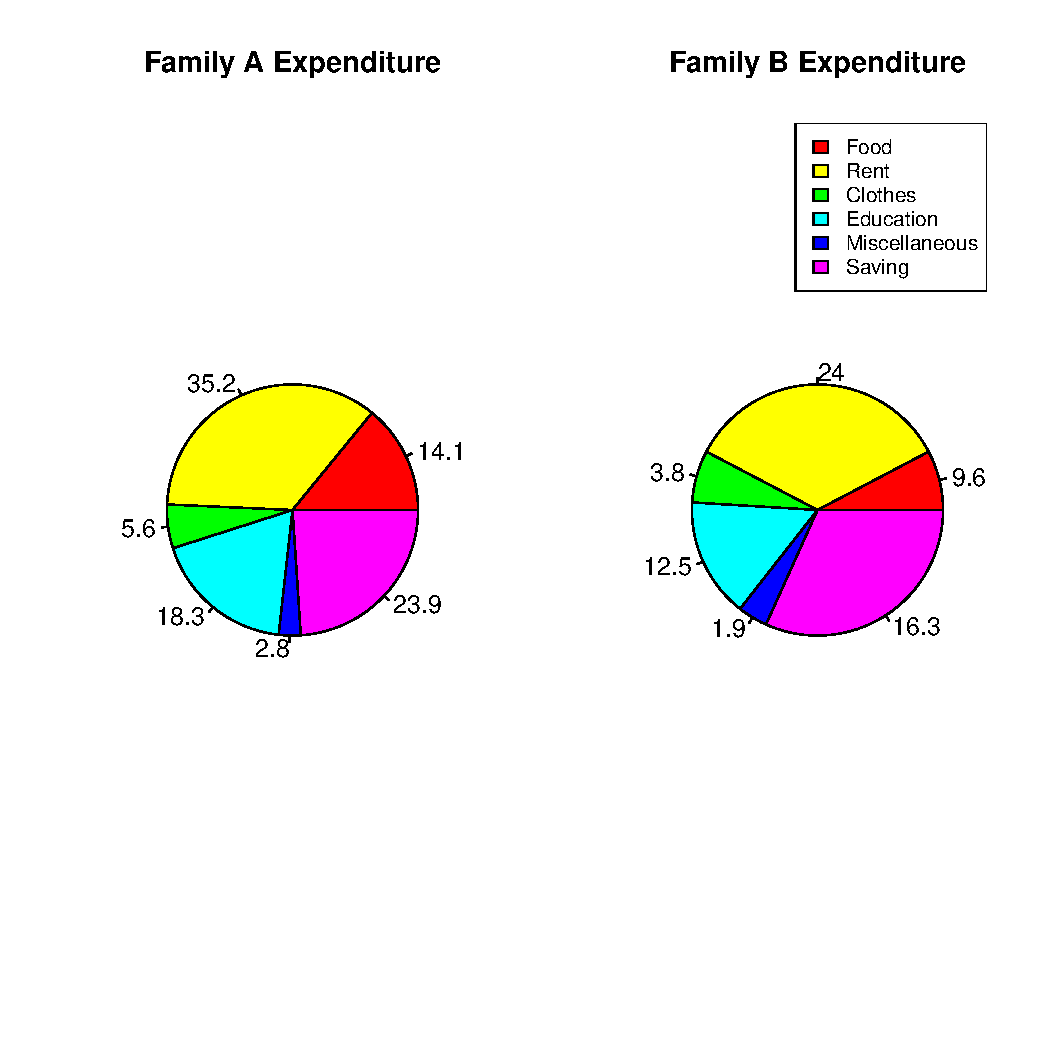
\includegraphics[width=\maxwidth]{figure/unnamed-chunk-1-1} 
\end{knitrout}
\newpage

\begin{knitrout}
\definecolor{shadecolor}{rgb}{0.969, 0.969, 0.969}\color{fgcolor}\begin{kframe}
\begin{alltt}
\hlcom{# Q2}

\hlcom{# 2.1 Display the number of variables in dataset}

\hlkwd{library}\hldef{(MASS)}
\hlkwd{data}\hldef{(}\hlsng{"Boston"}\hldef{)}
\hlkwd{ncol}\hldef{(Boston)}
\end{alltt}
\begin{verbatim}
## [1] 14
\end{verbatim}
\begin{alltt}
\hlcom{# 2.2 Draw a box plot for any two variables}
\hlkwd{boxplot}\hldef{(crim} \hlopt{~} \hldef{rad,}\hlkwc{data}\hldef{=Boston,} \hlkwc{varwidth} \hldef{=} \hlnum{TRUE}\hldef{,} \hlkwc{log}\hldef{=}\hlsng{'y'}\hldef{,} \hlkwc{las} \hldef{=} \hlnum{1}\hldef{)}
\hlkwd{title}\hldef{(}\hlsng{"Box plot of crim and rad"}\hldef{)}
\end{alltt}
\end{kframe}
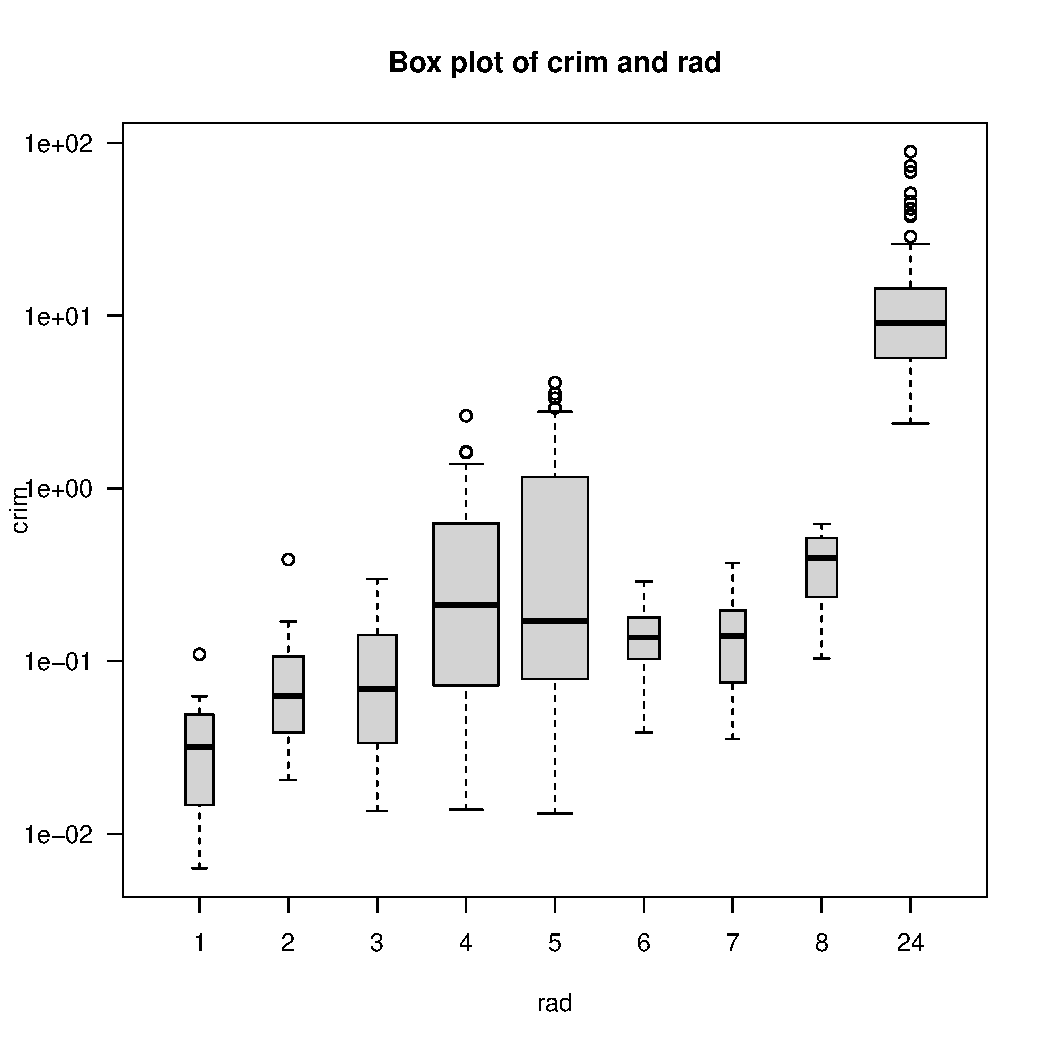
\includegraphics[width=\maxwidth]{figure/unnamed-chunk-2-1} 
\begin{kframe}\begin{alltt}
\hlcom{# 2.3 Scatterplot for any two variables\textbackslash{}}
\hlkwd{attach}\hldef{(Boston)}
\hlkwd{plot}\hldef{(age, dis ,} \hlkwc{main}\hldef{=}\hlsng{"AGE / DIS graph"}\hldef{,}\hlkwc{xlab}\hldef{=}\hlsng{"Age"}\hldef{,} \hlkwc{ylab}\hldef{=}\hlsng{"dis"}\hldef{,}\hlkwc{pch}\hldef{=}\hlnum{19}\hldef{)}
\end{alltt}
\end{kframe}
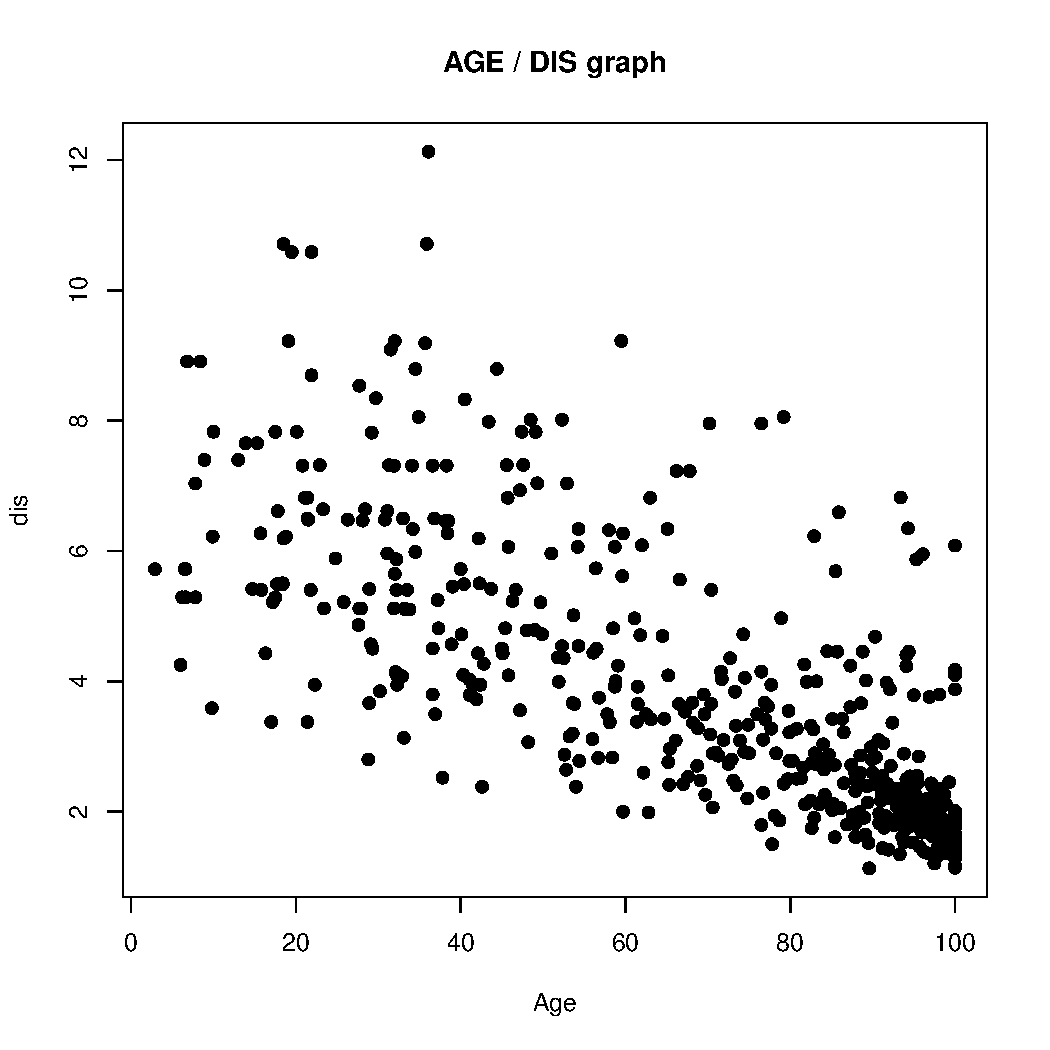
\includegraphics[width=\maxwidth]{figure/unnamed-chunk-2-2} 
\end{knitrout}

\end{document}
